\section{Models of Core and Programs}
\label{sec:model:core}
This section presents the automaton used to model a core, and the manner in
which programs are modeled.

\begin{figure}[hbt!]
\begin{center}
\begin{tabular}{c}
\begin{lstlisting}
const program_line_t program_101 [7] =
   {
      {INSTR_LOAD,    4, 0, 0},
      {INSTR_LOAD,    5, 0, 0},
      {INSTR_STORE,   6, 0, 0},
      {INSTR_LOAD,    6, 0, 0},
      {INSTR_STORE,   4, 0, 0},
      {INSTR_EVICT,   4, 0, 0},
      {INSTR_END,     0, 0, 0}
   };
\end{lstlisting}

\end{tabular}
\end{center}
\caption{Example of Program}
\label{fig:UPPAAL:program}
\end{figure}

Programs are sequences of instructions, without any jumps or branchings. The
available operators are \lstinline{INSTR_LOAD} (\loadinstr{}),
\lstinline{INSTR_STORE} (\storeinstr{}), \lstinline{INSTR_EVICT}
(\evictinstr{}), and \lstinline{INSTR_END} (signaling the end of the program).
Each operator targets a memory element, specified by its address.

\begin{definition}[Instruction Model]
Instructions are modeled by $\langle \texttt{instr}, \texttt{addr},
\texttt{min\_calc\_time}, \allowbreak{} \texttt{max\_calc\_time} \rangle$
tuples, with \texttt{instr} corresponding to the operator, \texttt{addr} the
targeted memory element, and \texttt{min\_calc\_time} and
\texttt{max\_calc\_time} define the interval during which the core is busy
following the instruction, with 0 indicating that the default CPU cycle time
should be used (a value set in the model parameters indicated in
Appendix~\ref{app:model_parameters}).
\end{definition}
\begin{example}[Instruction Model]
\lstinline!{INSTR_STORE, 42, 3, 9}! would indicate a \storeinstr{} applied to
the memory element $42$, and that after emitting this request, the core would
become unavailable for between 3 and 9 time units.
\end{example}

Figure~\ref{fig:UPPAAL:program} shows an example of program model.

All cores share the same automaton template, model's system description
initializes each core by passing as a parameter an integer corresponding to the
program they are to run.  The program number 0 is reserved, and indicates a
program made of random instructions.

\begin{figure}[hbt!]
\begin{center}
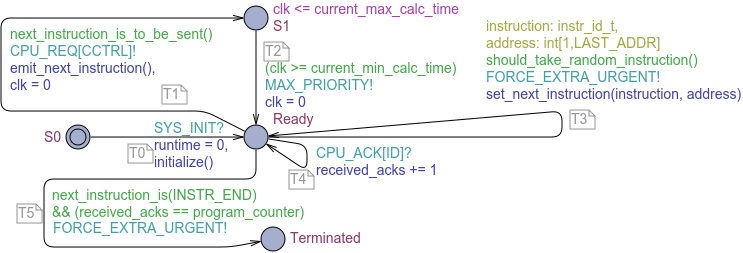
\includegraphics[width=0.9\textwidth]{\chapterdirectory/figure/Core.pdf}
\end{center}
\caption{Automaton for a Core}
\label{fig:UPPAAL:Core}
\end{figure}
Figure~\ref{fig:UPPAAL:Core} shows the automaton representing a core.

A core automaton has the following internal variables and clocks:
\paragraph{Clocks \& Variables for Core}
\begin{itemize}
\item
   \lstinline!clk! is a clock used to control the time spent being busy once
   an instruction has been sent.
\item
   \lstinline!runtime! is a clock measuring time since the moment the core
   performed its initialization.
\item
   \lstinline!program_counter! is an integer corresponding to the index of the
   next instruction in the program's array. It is updated by
   \lstinline!emit_next_instruction()!.
\item
   \lstinline!current_program_line! contains a copy of the current instruction
   line. Indeed, each program is stored in its own array, and since pointers are
   not available in UPPAAL, finding the current instruction line requires a
   chain of \lstinline!if!/\lstinline!else! tests so that the right array is
   selected before the \lstinline!program_counter! can be used as index. Thus,
   to optimize, the instruction line is search for once, then copied to
   \lstinline!current_program_line!. This variable is updated and used by all
   functions of this automaton.
\item
   \lstinline!current_max_calc_time! and \lstinline!current_min_calc_time!
   correspond to the maximal and minimal time the core remains inactive after
   sending an instruction.
\item
   \lstinline!received_acks! is a count of the number of the acknowledgments
   received from caches, which indicate that an instruction sent has been
   completed.
\item
   \lstinline!has_taken_random_instruction! indicates whether the current
   instruction line was randomly generated. This is used by both all functions
   in the $T_3$ transition.
\end{itemize}
%\end{varandclocks}

The automaton in Figure~\ref{fig:UPPAAL:Core} starts in the $S_0$
location, wherein it awaits the \textbf{SYS\_INIT} broadcast.

\paragraph{Transitions for Core}
\begin{description}
\item[$S_0 \automatatransitiontrace{T_0}{} \texttt{Ready}$]
   Upon synchronization on the \textbf{SYS\_INIT} broadcast channel,
   the core resets the \lstinline!runtime! clock and sets the
   \lstinline!current_program_line! variable to the value of the first
   instruction of the program and also updates the
   \lstinline!current_max_calc_time! and \lstinline!current_min_calc_time!
   variables accordingly.
\item[$\texttt{Ready} \automatatransitiontrace{T_1}{} S_1$]
   For the $T_1$ transition to be available, the next instruction has to
   correspond to a memory access (i.e. \loadinstr{},
   \storeinstr{}, \evictinstr{}). Furthermore, if the model requires all
   previous requests of a core to be completed prior to sending new ones,
   \lstinline!received_acks! must be equal to \lstinline!program_counter!.
   The $T_1$ transition sets the information passing shared variable to match
   the current instruction, then synchronizes the core's target cache
   \textbf{CPU\_REQ} sub-channel, thus transmitting the request to the cache.
   The core automaton also increment the program counter and updates its local
   variables with the data from the next instruction line.
\item[$S_1 \automatatransitiontrace{T_2}{} \texttt{Ready}$]
   After having sent an instruction, the core automaton stays waiting in the
   $S_1$ location for a time in the interval defined by
   \lstinline!current_max_calc_time! and \lstinline!current_min_calc_time!.
\item[$\texttt{Ready} \automatatransitiontrace{T_4}{} \texttt{Ready}$]
   The core's cache will synchronize on the core's \textbf{CPU\_ACK} sub-channel
   to signal completion of a request. This simply increments the
   \lstinline!received_acks! counter.
\item[$\texttt{Ready} \automatatransitiontrace{T_3}{} \texttt{Ready}$]
   A special case is when the program is random. The next instruction is
   randomly chosen by the $T_3$ transition. The
   \lstinline!current_max_calc_time! and \lstinline!current_min_calc_time! are
   kept to their default value. Furthermore, the
   \lstinline!has_taken_random_instruction! ensures that once a random
   instruction has been chosen, it is acted upon before a new one is chosen.
\item[$\texttt{Ready} \automatatransitiontrace{T_5}{} \texttt{Terminated}$]
   If the next instruction indicates the end of the program
   (\lstinline!INSTR_END!), and all sent requests have been acknowledged as
   completed. The core automaton uses the $T_5$ to enter the \texttt{Terminated}
   location, which completes its execution.
\end{description}
